% \documentclass[aps,11pt,citeautoscript,reprint]{revtex4-1}
\documentclass[aps,twocolumn,10pt,reprint]{revtex4}
\usepackage{graphicx}
\usepackage{epsfig}
\usepackage{amsmath}
\usepackage{graphicx}% Include figure files
\usepackage{dcolumn}% Align table columns on decimal point
\usepackage{bm}% bold math
\usepackage{amssymb}
\usepackage{amsmath}
\usepackage{epsf}
\usepackage{subfigure}
\usepackage{epstopdf}
\usepackage{color}
\usepackage{subeqnarray}
\usepackage{mathrsfs}
\usepackage[colorlinks=true, pdfstartview=FitV, linkcolor=red, citecolor=blue, urlcolor=blue]{hyperref}





\newcommand{\be}{\begin{equation}}
\newcommand{\ee}{\end{equation}}
\newcommand{\ben}{\begin{eqnarray}}
\newcommand{\een}{\end{eqnarray}}


\begin{document}



\title{Lab -1}


\author{name1 (ID1)}\email{ID1@daiict.ac.in}
\affiliation{Dhirubhai Ambani Institute of Information \& Communication Technology, Gandhinagar, Gujarat 382007, India\\ CS-302, Modeling and Simulation}
\author{name1 (ID2)}\email{ID2@daiict.ac.in}
\affiliation{Dhirubhai Ambani Institute of Information \& Communication Technology, Gandhinagar, Gujarat 382007, India\\ CS-302, Modeling and Simulation}

% abstract should mention what is done in the lab and the key observation 
\begin{abstract}

In this lab we numerically and analytically analyze the simple harmonic motion of a spring-mass system for different values of the frequency. We also look at the impact of different kinds of external impulse of the system. Our main observations are that.....   

\end{abstract}
\maketitle
% Introduction should give a brief background of the problem in your own words. Any references used should be cited
\section{Introduction}
Many systems in sciences and engineering show the property of small amplitude oscillations around a fixed position\cite{Ei35}. In the simplest approximation such motions can be modeled as a spring-mass system in which on one end of the spring is a rigid support and on the other is a mass. The dynamics depend on both the mass and the flexibilit of the spring \cite{Sh06}. ...... 
\section{Model}
Discuss the model in detail. This is the section where one checks the understanding of the model and the type of assumptions that have been used. If there are equations then write and discuss the equations. As example,

% equation should be labelled and properly referenced in the text
\be\label{Eq:SHM}
\ddot{x} = -\omega^{2}x + f(t)
\ee


Eq.~(\ref{Eq:SHM}) represents the standard equation of a simple harmonic motion with $\omega$ being the natural frequency and $f(t)$ is a time dependent external driving force. Notice that no dissipative effects have been included and the small angle approximation has been invoked implying that we retain the lowest order term in the Taylor series expansion of the force around the equilibrium position. The solution in the absence of any driving $f(t) = 0$ is 

\be\label{Eq:SHMSol}
x(t) = A \cos\left(\omega t + \phi\right)
\ee


\section{Results}

Fig.~\ref{Fig:shm} shows the typical evolution of the position of the oscillator. Periodic motion is indeed observed etc... Discuss your results in the most intuitive way. What is that you see, why in your opinion the system shows this behavior etc. Figure caption is important and should be self explanatory. Figure label and legend if any should be clear. Show only the relevant part of your results unless there is something that you want to discuss in the non relevant part. How you showcase your result is also important. For instance if you want to show the peak amplitude as a function of the maximum value of the driving force then you should make a figure with such details.
\begin{figure}[!h]
\centering
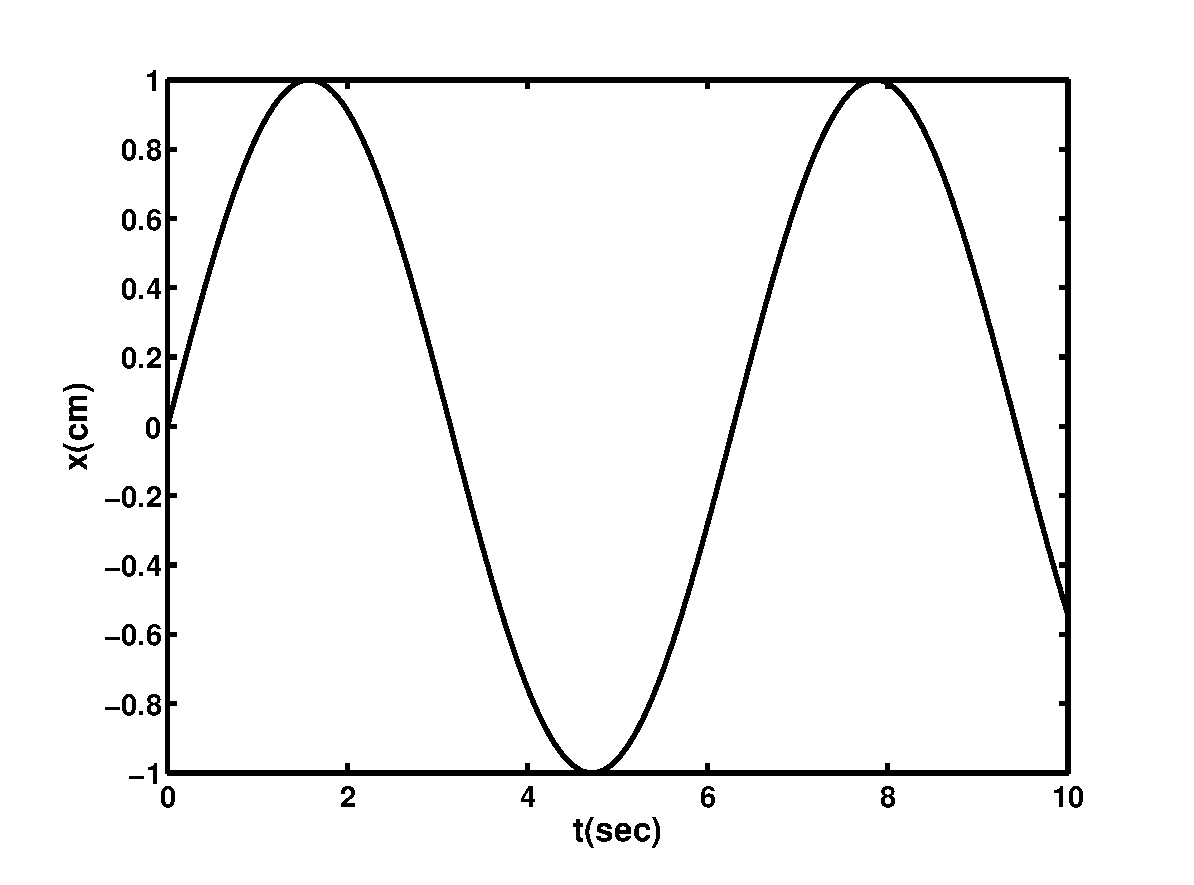
\includegraphics[width = 3.50 in]{shm}~
\caption{Typical evolution of the position with time for the simple harmonic oscillator. The initial conditions are $x_{0} = 0$ and $v_{0} = \sqrt{2}$. The constant $\omega =1$.}\label{Fig:shm}
\end{figure}
\section{Conclusions}
In conclusion, we have studied a simple mathematical model of a system which shows oscillatory behavior. Discuss your study in a simple way such that a reader would know what has been achieved by the analysis that has been carried out. 

\begin{thebibliography}{}
% if citing a book mention the name of the authors, book title, Publisher and year
\bibitem{Sh06} A. Shiflet and G. Shiflet, {\it Introduction to Computational Science: Modeling an Simulation for the Sciences}, Princeton University Press.3, 276 (2006).
% if citing papers you should mention the authors, journal name volume, page number and year
\bibitem{Ei35} A. Einstein and N. Rosen, Phys. Rev.{\bf 48}, 73 (1935).
\end{thebibliography}


\end{document}